\documentclass{plainbook}

\usepackage{amsfonts}
\usepackage{amsmath}
\usepackage{amssymb}
\usepackage{hyperref}
\usepackage{svg}
\usepackage{booktabs}
\usepackage{framed}


% font; do not use in overleaf

\usepackage[UTF8,scheme=plain,fontset=none]{ctex}
    \setCJKmainfont[BoldFont={Source Han Serif SC-SemiBold},ItalicFont={FZKai-Z03}]{FZShuSong-Z01}
    \setCJKsansfont[BoldFont={Source Han Serif SC-SemiBold}]{FZKai-Z03}
    \setCJKmonofont[BoldFont={Source Han Serif SC-SemiBold}]{FZFangSong-Z02}
    \setCJKfamilyfont{zhsong}{FZShuSong-Z01}
    \setCJKfamilyfont{zhhei}{Source Han Serif SC-SemiBold}
    \setCJKfamilyfont{zhkai}[BoldFont={Source Han Serif SC-SemiBold}]{FZKai-Z03}
    \setCJKfamilyfont{zhfs}[BoldFont={Source Han Serif SC-SemiBold}]{FZFangSong-Z02}


\title{晨沐公的数学习题集}

% Set the authors of the book (multiple authors separated by \and).
\author{bilibili:晨沐公Johnny \quad github: MATHhahetaDEATH}

% Set the date to the current date.
\date{\today}

% customised commands
\definecolor{winered}{rgb}{0.5,0,0}
\newcommand{\xl}[1]{\overrightarrow{#1}}
\newcommand{\nd}[1]{〔#1〕}
\newcommand{\ssb}[1]{\big( #1 \big)}
\newcommand{\R}{\mathbb{R}}
\newcommand{\C}{\mathbb{C}}
\newcommand{\Z}{\mathbb{Z}}
\newcommand{\F}{\mathbb{F}}
\newcommand{\lmap}{\mathcal{L}}
\newcommand{\mmatrix}{\mathcal{M}}
\newcommand{\sw}[1]{\boxed{\text{解法 #1}} \ }
\newcommand{\buzhou}[1]{$#1^{\circ} \ $}
\usepackage{ulem}
	\newcommand{\tk}{\uline{\hspace{4em}}}
\newcommand{\pspace}{\vspace{0.5em}}
\usepackage{amsmath,amsfonts}
	\DeclareMathOperator{\spn}{span}
	\DeclareMathOperator{\card}{card}
	\DeclareMathOperator{\ic}{i}
	\DeclareMathOperator{\arccot}{arccot}
	\DeclareMathOperator{\setjianfa}{\textbackslash}
	\DeclareMathOperator{\nul}{null}
	\DeclareMathOperator{\rge}{range}
	\DeclareMathOperator{\sgn}{sgn}

% Begin the document.
\begin{document}

% Front matter section.
\frontmatter

% Include the title page, which is located in the FrontMatter subfolder.
% This code snippet creates a title page for a book.

% The 'titlepage' environment starts the title page.
\begin{titlepage}
    % The 'colorbox' is used to create a colored background for the book title and subtitle.
    % 'black!5' sets the color to 5% black (a light gray shade).
    \colorbox{black!5}{
        % The first 'parbox' is used to center the title and subtitle within the colored background.
        \parbox[t]{0.975\textwidth}{%
            % The second 'parbox' is used to center the title and subtitle text.
            \parbox[t]{0.95\textwidth}{%
                % Right-align the title and subtitle text, and set it in uppercase and huge font size.
                \raggedleft\vspace{0.75cm}\Huge\scshape
                代数笔记 \\[7.5pt]
                \large\bf Algebra
                \vspace{0.75cm}
            }
        }
    }

    % Vertically space the content evenly, pushing the text to the center of the page.
    \vfill

    % The first 'parbox' is used to display horizontal rules on both sides of the authors' information.
    \parbox[t]{0.95\textwidth}{%
        % Right-align the horizontal rule and add some vertical space above and below it.
        \hfill\rule{0.15\linewidth}{0.5pt}\\[7.5pt]
        % Right-align the authors' names and affiliations.
        \raggedleft
        \textcopyright\:{晨沐公\textsuperscript{\textdagger}}\\[4pt]
        
        % Display the superscript \textdagger symbol and authors' affiliations.
        \normalsize\textsuperscript{\textdagger} 成都市锦江区嘉祥外国语高级中学\\

        % Right-align the second horizontal rule.
        \hfill\rule{0.15\linewidth}{0.5pt}
    }
\end{titlepage}


% Create the book's title page.
\maketitle\pagebreak

% Include the dedication page from the FrontMatter subfolder.
% % This code snippet creates a centered dedication page with two authors' names.

\begin{center}
    % The dedication page has no page number (empty page style).
    \thispagestyle{empty}
    
    % Vertically space the content evenly, pushing the text to the center of the page.
    \vspace*{\fill}
    
    % First author's dedication text in italics.
    \textit{To my someone and someone}
    
    % The first author's name is right-aligned and set in sans-serif small caps.
    \begin{flushright}
        {\sffamily\scshape First Author}
    \end{flushright}
    
    % Add some vertical space between the first and second author.
    \bigskip
    
    % Second author's dedication text in italics.
    \textit{To my someone and someone}
    
    % The second author's name is right-aligned and set in sans-serif small caps.
    \begin{flushright}
        {\sffamily\scshape Second Author}
    \end{flushright}
    
    % Vertically space the content evenly again, pushing any remaining space to the bottom of the page.
    \vspace*{\fill}
\end{center}


% Include the epigraph page from the FrontMatter subfolder.
% This code snippet creates a quote block attributed to an author.

% Vertically space the content evenly, pushing the quote to the center of the page.
\vspace*{\fill}

% Set the font size to \Large (large) and the text style to italics.
\Large\textit{It is not from the benevolence of the butcher, the brewer, or the baker, that we expect our dinner, but from their regard to their own interest. }

% Add some vertical space after the quote.
\bigskip

% The author's name is right-aligned and set in sans-serif small caps.
\begin{flushright}
    \sffamily\scshape Adam Smith
\end{flushright}

% Set the font back to the default (normal font size and style).
\normalfont\normalsize

% Vertically space the content evenly again, pushing any remaining space to the bottom of the page.
\vspace*{\fill}


% Include the foreword page from the FrontMatter subfolder.
\chapter*{前言}

本讲义的大致结构基于Zorich的教材, 作者本着易于理解的原则做了一些调整. 

参考书目如下: 

\begin{enumerate}

\item
B.A.卓里奇.
\newblock {\em 数学分析(第一卷)}.
\newblock 高等教育出版社, 2019.

\item
B.A.卓里奇.
\newblock {\em 数学分析(第二卷)}.
\newblock 高等教育出版社, 2019.

\item
清华大学数学系及丘成桐数学科学中心.
\newblock {\em
  数学分析之课程讲义(丘成桐数学英才班试用)}.
\newblock 2020.

\item
Ayumu.
\newblock {\em 数学分析I}.
\newblock 复旦大学出版社, 2024.

\item
Ayumu.
\newblock {\em 数学分析II}.
\newblock 2024.

\item
Ayumu.
\newblock {\em 数学分析III}.
\newblock 2024.

\item
陈天权.
\newblock {\em 数学分析讲义(第一册)}.
\newblock 北京大学出版社, 2009.

\item
陈天权.
\newblock {\em 数学分析讲义(第二册)}.
\newblock 北京大学出版社, 2010.

\item
陈天权.
\newblock {\em 数学分析讲义(第三册)}.
\newblock 北京大学出版社, 2010.

\item
汪林.
\newblock {\em 数学分析中的问题和反例}.
\newblock 高等教育出版社, 2015.

\end{enumerate}


% Include the preface page from the FrontMatter subfolder.
% \chapter*{序}



\undersign

% Include the acknowledgement page from the FrontMatter subfolder.
% \chapter*{致谢}



\undersign

% Table of contents page.
\tableofcontents

% Main matter section.
\mainmatter


\chapter{行列式}









\chapter{矩阵的运算}









\chapter{矩阵的相抵与相似}







\chapter{二次型, 矩阵的合同}





\chapter{向量空间与线性映射}





\chapter{具有度量的向量空间}







\chapter{多重线性代数}

\chapter{数学分析 Analysis}

% 数据损坏了一部分

\section{集合论与可数集}

\begin{exercise}{用归纳集构造自然数}
	对于集合$x$, 称$x$的\textit{后继}为$x^+ := x \cup \{ x \}$. 若一个集合包含空集和自身任何一个元素的后继(无穷公理说明这样的集合是存在的), 则称其为一个\textit{归纳集}. 定义自然数集$N_0$为所有归纳集的交集. 

	若将$\cdot \mapsto \cdot ^{+}$视作映射$S:N_0 \to N_0$, 下面证明这个映射符合Peano公理. 

	1) $x=y \Rightarrow x^+=y^+$, 即该映射是良好定义的. 

	2) $\forall x \in N_0,~x^+ \neq \varnothing$, 即$\varnothing \notin S(N_0)$. 

	3) $(A \subseteq N_0) \wedge (\varnothing \in A) \wedge (\forall x \in A,~x^+ \in A) \Rightarrow A=N_0$, 即如果自然数集的子集也是归纳集, 那么该子集就是自然数集本身(数学归纳原理). 

	4) $x^+=y^+ \Rightarrow x=y$, 即$S$是一个单射.
\end{exercise}
\begin{solution}
	假设$x\neq y$但$x \in (x \cup \{ x \})=(y \cup \{ y \})$, 从而$x \in \{ y \}$(舍)或$x \in y$. 同理$y \in x$. 下面证明, 若$x \in y$, 则$x \subseteq y$, 从而结束证明.
	
	固定$x$, 对$y$归纳证明(这相当于利用3)): 当$y= (\varnothing )^+=\{ \varnothing \}$时, 若$x \in y$则$x = \varnothing$, 显然$x \subseteq y$; 设$x \in y$则$x \subseteq y$, 下证若$x \in y^+=y \cup \{ y \}$则$x \subseteq y^+$. 分类讨论. 当$x=y$时显然成立, 当$x \in y$时由归纳假设可知$x \subseteq y$, 从而$x \subseteq y^+$. 
\end{solution}

\begin{exercise}{$\R$不可数-对角线方法}
	利用对角线方法, 证明区间$(0,1)$是不可数的. (从而证明$\R$是不可数的)
\end{exercise}
\begin{solution}
	设$(0,1)$可数,记$(0,1)-\{ x/9:x \in \mathbb{Z}, 1 \leq x \leq 8 \}=\{ a_1, a_2, \cdots ,a_n ,\cdots \}$,并令$a_i$的十进制小数表示为$a_i=0.k_{i1}k_{i2}\cdots$.构作如下无限矩阵:
	
	$$\begin{pmatrix}
 \color{red} k_{11} & k_{12} & k_{13} & \cdots & k_{1m} & \cdots \\
 k_{21} & \color{red} k_{22} & k_{23} & \cdots & k_{2m} & \cdots \\
 k_{31} & k_{32} & \color{red} k_{33} & \cdots & k_{3m} & \cdots \\
 \vdots & \vdots & \vdots & \color{red} \ddots & \vdots & \cdots \\
 k_{m1} & k_{m2} & k_{m3} & \cdots & \color{red} k_{mm} & \cdots \\
 \vdots & \vdots & \vdots & \vdots & \vdots & \color{red} \ddots
\end{pmatrix}.$$

	选取对角线上的数码$k_{11},k_{22},\cdots $.现在任取$k_j \neq k_{jj}$使得$1 \leq k_j \leq 8$.(假设不存在满足不等的$k_j$,则$a_j$小数点后数码均相同,必然为$\{ x/9:x \in \mathbb{Z}, 1 \leq x \leq 8 \}$中某个元素,矛盾).
	
	构造$a=0.k_1k_2k_3\cdots$,由上面的构造可知$a$的十进制小数表示唯一,又因为存在$m$使得$a=a_m$,可得$k_m=k_{mm}$,矛盾.
\end{solution}

\begin{exercise}{$\R$不可数-闭区间套}
	利用闭区间套定理证明$\R$是不可数的. 
\end{exercise}
\begin{solution}
	假设可将$\R$写作$\{ x_1,x_2,\cdots \}$. 取$a_1<x_1<b_1$, 那么在$[a_1, \frac{2}{3}a_1+\frac{1}{3}b_1], [\frac{2}{3}a_1+\frac{1}{3}b_1, \frac{1}{3}a_1+\frac{2}{3}b_1], [\frac{1}{3}a_1+\frac{2}{3}b_1 , b_1]$中至少有一个区间不包含$x_1$, 记为$I_1=[a_2,b_2]$. 递归地定义$I_n$, 则$I_1 \supseteq \cdots \supseteq I_n \supseteq \cdots$且$|I_n| \to 0$. 那么存在唯一的$x \in \bigcap_{n \geq 1}I_n$, 即$x \notin \R$, 矛盾. 
\end{solution}

%-----------------------------------------------

\clearpage
\section{实数定义, 数列极限, 数项级数}

\subsection{实数完备性定理的互推}

\begin{exercise}{Dedekind定理}
	用Dedekind分割的定义证明Dedekind定理: \textit{$\R$上任一Dedekind分割的上集均有最小元素. }
\end{exercise}
\begin{solution}
	记该分割为$\alpha ' \mid \beta '$. 我们想要证明, $\beta '$的最小元素对应某个实数, 确切地说是对应一个$\mathbb{Q}$上的Dedekind分割$\alpha \mid \beta$, 其中$\alpha , \beta$分别表示由$\alpha '$和$\beta '$中所有有理数构成的集合.
	
	(i)根据上述定义, $\alpha$显然向下封闭.由于$\alpha '$中无最大元素, 任取$a \in \alpha$都存在$M \in \alpha '$使得$a < M$. 由推论2.1可知, 存在有理数$m$使得$a<m<M$.即得$\alpha$中亦无最大元素, 所以$\alpha \mid \beta$是$\mathbb{Q}$上的一个Dedekind分割.
	
	(ii)将$\alpha$看做实数, 假设$\alpha \in \alpha '$, 同上易知存在另一个($\mathbb{Q}$上的)上集$\alpha _1$满足$\alpha < \alpha _1$. 将$\alpha _1$看做有理数可知, 其一定在$\beta$内, 所以作为上集的$\alpha _1 \in \beta '$, 矛盾.
	
	(iii)同(ii)可得, $\alpha$是$\beta '$的最小元素.
\end{solution}

\begin{exercise}{Dedekind定理$\to$确界原理}
	用Dedekind定理证明确界原理: \textit{设非空集合$X \subseteq \R$.若其存在上界, 则一定存在上确界. }
\end{exercise}
\begin{solution}
	若$X$中存在最大元素, 则显然其上确界为该最大元素.假设$X$中不存在最大元素, 设其上界组成集合$\beta$, 取$\alpha = \beta ^c$.容易证明$\alpha \mid \beta$是$\R$上的一个Dedekind分割, 从而由Dedekind定理可得$\beta$存在最小元素, 即为$X$的上确界.
\end{solution}

\begin{exercise}{确界原理$\to$Dedekind定理}
	用确界原理证明Dedekind定理. 
\end{exercise}
\begin{solution}
	取$\R$上的Dedekind分割$\alpha \mid \beta$, 显然$\alpha$中的每个元素都是$\beta$的下界.那么由确界原理可知$\beta$存在下确界.
	
	假设$\inf \beta$不是$\beta$的最小元素, 即$\inf \beta \notin \beta$, 则$\inf \beta \in \alpha$.由于存在$x \in \alpha$使得$x > \inf \beta$, 故$x \in B$, 矛盾. 
\end{solution}

\begin{exercise}{确界原理$\to$Heine-Borel定理}
	用确界原理证明Heine-Borel定理: \textit{ 对于给定闭区间,任何一个能够覆盖它的开区间族必然包含一个亦可覆盖它的有限子族. }
\end{exercise}
\begin{solution}
	设$E=\{ x \in [a,b]:[a,x]\text{存在一个$S$的有限子覆盖} \}$. 显然存在$I_0 \in S$满足$a \in I_0$, 故存在$x_0 \in I_0$使得$x_0>a$. 从而, $E$非空. 
	
	显然$b$是$E$的一个上界, 故$E$存在上确界且$\sup E \leq b$. 假设$\sup E < b$. 取开区间$I$使得$\sup E \in I$, 则存在$\delta >0$使得$I \supseteq N_{\delta}(\sup E)$, 那么$E$所确定的有限子覆盖族$\cup \{ I \}$可以覆盖$[a,\sup E+\delta]$, 这说明$\sup E+\delta \in E$, 矛盾. 
	
	现在证明$b \in E$. 假设$b \notin E$, 类似地取包含$b$的$I' \in S$, 容易得到$E$所确定的有限子覆盖族$\cup \{ I' \}$可以覆盖$[a,b]$. 
\end{solution}

\begin{exercise}{Heine-Borel定理$\to$确界原理}
	用Heine-Borel定理证明确界原理. 
\end{exercise}
\begin{solution}
	取不存在最大元素而存在上界$b$的集合$X$.假设$X$没有上确界.任取$a \in X$,构造$S=\{ N_{\delta}(x):x \in [a,b] \}$,其中$\delta$满足:
	
	(i)当$x$是$X$的上界时,总存在另一个上界$x'$使得$x'<x$,此时记$\delta =x-x'$;
	
	(ii)当$x$不是$X$的上界时,存在$x' \in X$使得$x'>x$,即$\delta = x'-x$.
	
	由Heine-Borel定理知存在$S$的一个有限子覆盖$S'$.考虑$S'$中所有(i)类的区间,取它们之中左端点的最小值$m$,可知$m$为$X$的上界,则存在另一个$m'<m$亦为$X$的上界,这样的$m$不可能在(i)中,即得矛盾.
\end{solution}

\begin{exercise}{确界原理$\to$单调收敛定理}
	用确界原理证明单调收敛定理: \textit{单调不减数列$\{ x_n \}$收敛于$\sup \{ x_n \}$当且仅当其有上界. }
\end{exercise}
\begin{solution}
	只证明充分性:若$\{ x_n \}$存在上界,则其存在上确界$\sup \{ x_n \}$,意即对任意的$\varepsilon$都存在$N$使得$\sup \{x_n\}-\varepsilon < x_N \leq \sup \{ x_n \}$.取$n>N$可知$$\sup \{x_n\}-\varepsilon < x_N \leq a_n \leq \sup \{ x_n \}.$$
	这表明$\{ x_n \}$收敛于$\sup \{ x_n \}$.
\end{solution}

\begin{exercise}{单调收敛定理$\to$闭区间套定理}
	用单调收敛定理证明闭区间套定理: \textit{设闭区间$I_n=[a_n,b_n]$,若$I_1 \supseteq I_2 \supseteq \cdots $,且$\lim_{n\to \infty} (a_n-b_n)=0$,则存在唯一的$c$属于所有闭区间. }
\end{exercise}
\begin{solution}
	显然$\{ a_n \},\{ b_n \}$均单调且有界,故存在极限.注意到$\lim_{n\to \infty} a_n = \lim_{n\to \infty} b_n$,记为$c$,即$\sup \{ a_n \} = \inf \{ b_n \} = c$,从而对任意$n$都有$a_n \leq c \leq b_n$,存在性即得证.
	
	现假设存在不同的$c'$亦满足$a_n \leq c' \leq b_n$对所有$n$都成立,那么$c' \leq \lim_{n\to \infty} b_n = \lim_{n\to \infty} a_n \leq c$,同理$c \leq c'$,即得$c=c'$,矛盾.
\end{solution}

\begin{exercise}{闭区间套定理$\to$Bolzano-Weierstrass定理}
	用闭区间套定理证明Bolzano-Weierstrass定理: \textit{有界无限实数列必有收敛子列.}
\end{exercise}
\begin{solution}
	设有界数列$\{ x_n \}$. 对于任意的$x_n$总存在$a \leq x_n \leq b$. 显见区间$[a,\frac{a+b}{2}]$和$[\frac{a+b}{2},b]$中必有至少一个含有$\{ x_n \}$的无穷多项. 取之, 记为$I_0$. 重复该过程得到$I_0 \supseteq I_1 \supseteq \cdots I_n \supseteq \cdots$. 注意到$I_n$的长度为$\frac{b-a}{2^n} \to 0$, 由闭区间套定理可得存在唯一的$c \in I_n~(n=0,1,\cdots)$. 只需依次在$I_j$中取一个$x_{k_j}$即构成收敛于$c$(容易证明)的数列$\{ x_{k_n} \}$. 
\end{solution}

\begin{exercise}{Bolzano-Weierstrass定理$\to$Cauchy收敛准则}
	用Bolzano-Weierstrass定理证明Cauchy收敛准则: \textit{一个数列收敛当且仅当它是一个Cauchy列. }
\end{exercise}
\begin{solution}
	必要性:设数列$\{ x_n \}$收敛于$A$.则对任意$\varepsilon >0$都存在足够大的$m,m$满足$|x_m-A|<\varepsilon ,|x_n-A|<\varepsilon$,从而可得$|x_m-x_n|<|x_m-A|+|x_n-A|<2\varepsilon$对足够大的$m,n$成立.
	
	充分性:易证Cauchy列$\{ x_n \}$一定有界.由Bolzano-Weierstrass定理可知$\{ x_n \}$存在某个子列$\{ x_{n_k} \}$有极限$A$.对任意$\varepsilon >0$,当$n_k$足够大时有$|x_{n_k} - A|<\varepsilon$.从而当$n$足够大时有$|x_n-A|<|x_n-x_{n_k}|+|x_{n_k}-A|<2\varepsilon$.
\end{solution}

\begin{exercise}{Cauchy收敛准则$+$Archimedes性质$\to$确界原理}
	用Cauchy收敛准则(结合Archimedes性质)证明确界原理. 
\end{exercise}
\begin{solution}
	设非空集合$X$存在上界,由Archimedes性质可知,对任意的$n$都存在唯一的整数$k_n$使得$q_n=\frac{k_n}{n}$是$X$的上界而$\frac{k_n-1}{n}$不是.我们断言$\{ q_n \}$是一个Cauchy列,从而其存在极限$q$.这里的$q$显然是$X$的上界,而对每个$n$都存在$x \in X$使得$x>q_n-\frac{1}{n}$,容易得到$q$就是$X$的上确界.
	
	断言的证明:对任意的$m,n$分别存在$x_m,x_n \in X$使得$q_m-\frac{1}{m} < x_m,q_n-\frac{1}{n} < x_n$,而$q_m \geq x_n,q_n \geq x_m$,所以$|q_m-q_n|<\max \{ \frac{1}{m},\frac{1}{n} \}$,易知断言成立.
\end{solution}

\clearpage
\subsection{逼近}

\begin{exercise}{有理逼近}
	设无理数$\alpha$. 称$\alpha$可被有理逼近, 如果$\forall n,N \in \mathbb{N}^{*}, \exists p/q \in \mathbb{Q} \left(|\alpha - p/q | < \frac{1}{Nq^n} \right)$. 
	
	1) 证明: $\xi = \sum_{n=1}^{\infty} 10^{-n!} = \frac{1}{10} + \frac{1}{10^2} + \frac{1}{10^6}+\frac{1}{10^{24}} + \cdots$可被有理逼近. 
	
	2) (Liouville) 若$\alpha$可被有理逼近, 则其必然是超越数. 
\end{exercise}
\begin{solution}
	容易验证$\xi$作为一个级数的确是收敛的. 又$\xi$是一个无限不循环小数, 所以为无理数.
	
	考虑取$p_j/q_j = \sum_{n=1}^{\infty} 10^{-n!}$, 则有
	\begin{align*}
		\left| \xi - \frac{p_j}{q_j} \right| &= \sum_{n=j+1}^{\infty} 10^{-n!} = 10^{-(j+1)!} \sum_{n=j+1}^{\infty} 10^{(j+1)!-n!} < 10^{-(j+1)!} \sum_{k=0}^{\infty} \left( 10^{(j+1)!-(j+2)!} \right)^k \\
		&= \frac{1}{10^{(j+1)!} + 10^{-(j+1)}} < \frac{1}{10^{(j+1)!}}.
	\end{align*}
	令$q_j=10^{j!}$, 那么$|\xi - \frac{p_j}{q_j}| < \frac{1}{q_j^j}$. 
	
	接着, 固定$n$, 对于任意$N>0$, 取$r$使得$2^r>N$. 上面的计算说明存在$p/q$使得$|\xi - \frac{p}{q} |< \frac{1}{q^{r+n}} < \frac{1}{2^r q^n} < \frac{1}{Nq^n}$. 
\end{solution}
\begin{solution}
	假设$\alpha$是代数数, 设为$m$次整系数多项式$f(x) = a_0 + a_1x + \cdots + a_mx^m$的根. 下证存在特定的$n_m$和$N$使得对所有$p/q \in \mathbb{Q}$都有$|\alpha - p/q| > \frac{1}{Nq^{n_m}}$. 
	
	与a)类似, 我们考虑一个数列$\alpha _j = p_j/q_j \to \alpha$. 待定一个$\varepsilon$, 则存在$j$使得$|\alpha - \alpha _j |<\varepsilon$. 那么$$\frac{ f(\alpha _j)-f(\alpha) }{\alpha _j - \alpha}  = a_1 \cdot \frac{\alpha _j - \alpha}{\alpha _j - \alpha} + \cdots + a_m \cdot \frac{\alpha _j^m - \alpha ^m}{\alpha _j - \alpha}, $$
	其中$$\left| a_k \cdot \frac{\alpha _j^k - \alpha ^k}{\alpha _j - \alpha} \right| = |a_k(\alpha _j ^{k-1} + \alpha _j ^{k-2} \alpha + \cdots + \alpha ^{k-1})| < k|a_k|(|\alpha |+\varepsilon)^{k-1}$$
	对$k=1,\cdots ,m$成立. 因此$$\left| \frac{f(\alpha _j)}{\alpha _j - \alpha} \right| < \sum_{k=1}^{m} k|a_k|(|\alpha |+\varepsilon)^{k-1} =: M.$$
	$M$是一个仅与$\alpha ,\varepsilon$有关的常数. 那么$$\left|\alpha - \frac{p_j}{q_j}	\right| > \frac{|f(\alpha _j)|}{M} = \frac{1}{q_j^m} \cdot \frac{|a_0q_j^m + a_1p_jq_j^{m-1} + \cdots + a_{m-1}p_j^{m-1}q_j + a_mp_j^{m} |}{M}. $$
	注意到绝对值内必然是一个整数, 且$f(\alpha _j) \neq 0$ (否则消去$(x-\alpha _j)$之后可得$\alpha$是$m-1$次多项式的根), 所以绝对值整体最小值为$1$, 即$\left|\alpha - \frac{p_j}{q_j}	\right| > \frac{1}{Mq_j^m}$. 
	
	现在做一些小的调整. 
	
	首先, 之前待定的数列$\{ \alpha _j \}$和$\varepsilon >0$可以弱化为: 待定$\varepsilon$, 令$\{ \alpha _j \}$满足$|\alpha - \alpha _j |<\varepsilon$. 那么对这样的$\{ \alpha _j \}$我们完成了证明. 
	
	另一方面, 对于$\alpha ' \in \mathbb{Q} - \{ \alpha _j \}$, 必有$|\alpha ' - \alpha|>\varepsilon$. 取$\varepsilon = 1$即得$|\alpha ' - \alpha| > \frac{1}{q^n}$. 
\end{solution}

\begin{exercise}{连分数}
	给定自然数序列$\{ q_n \}$, 定义序列$\{ R_n \}$: $$R_1=q_1, R_2=q_1+\frac{1}{q_2}, \cdots ,R_n = q_1 + \dfrac{1}{q_2 
          + \dfrac{1}{q_3 
          + \cdots \dfrac{1}{q_{n-1}+\dfrac{1}{q_n}}  } }.$$
          
	1) 证明: 对每个有理数$\frac{m}{l}$, 均存在唯一的$n$和$\{ q_n \}$使得$R_n=\frac{m}{l}$. (提示: 利用Euclid算法)

	2) 渐进分数序列$\{ R_n \}$满足以下不等式: $$\exists m,l,~ R_1<R_3< \cdots <R_{2k-1} < \frac{m}{l} < R_{2k} < R_{2k-2} < \cdots < R_2.$$

	3) 每个无穷连分数(定义为数列$\{ R_n \}$的极限)都存在, 且为无理数. 

	4) 可以按照如下方式递归地构造$R_k$的分子$P_k$与分母$Q_k$. (对比Pell方程)
	$$P_1=q_1, P_2=q_1q_2+1, P_k=P_{k-1}q_k+P_{k-2}~(k \geq 3); $$
	$$Q_1=1, Q_2=q_2, Q_k=Q_{k-1}q_k+Q_{k-2}~(k \geq 3).$$

	5) $\frac{1+\sqrt{5}}{2}$的渐进分数$R_k=\frac{P_k}{Q_k}$满足$$\big| \frac{1+\sqrt{5}}{2} - \frac{P_k}{Q_k} \big|>\frac{1}{\sqrt{5} Q_k^2}, k \geq 1.$$
\end{exercise}

\clearpage
\subsection{数列极限}

\begin{exercise}{Cesàro求和极限} \label{exer:cesaro_limit}%yp p67 
	设$\{ a_n \}$是实数序列, 定义算术平均值序列$\sigma _n = \frac{a_1+\cdots + a_n}{n}, n \in \mathbb{N}^{*}$. 

	1) 设$\lim_{n\to \infty} a_n=a$, 则$\lim_{n\to \infty} \sigma _n=a$. 

	2) 设$n|a_{n+1}-a_n| \to 0$且$\lim_{n\to \infty} \sigma _n=a$, 则$\lim_{n\to \infty} a_n=a$. 

	3) 设$\{ n|a_{n+1}-a_n| \}$是有界的且$\lim_{n\to \infty} \sigma _n=a$, 则$\lim_{n\to \infty} a_n=a$. 
\end{exercise}
\begin{solution}
	记$b_k=a_{k+1}-a_k$. 设$k|b_k|<M$. 将所有的$\{ a_n \}$缩小$M$倍, 可以不妨设$M=1$. 
	
	待定$n>N$, 由于
	\begin{align*}
		&|n\sigma _n - N\sigma _N - (n-N)a_N| = |(a_{N+1}-a_N) + \cdots + (a_{n}-a_N)| = \big|\sum_{k=N}^{n-1} (n-k)b_k \big| \\
		&< \sum_{k=N}^{n-1} \frac{n-k}{k} < \left( \frac{n}{N}-1 \right) (n-N). 
	\end{align*}
	从而$$\big| a_N - \frac{n\sigma _n - N\sigma _N}{n-N} \big| < \frac{n}{N} - 1,$$
	即有$$-\left(\frac{n}{N}-1 \right) + \sigma _n + \frac{N}{n-N}(\sigma _n - \sigma _N) < a_N < \left(\frac{n}{N}-1 \right) + \sigma _n + \frac{N}{n-N}(\sigma _n - \sigma _N).$$
	待定$\varepsilon$, 令$n = \lfloor (1+\varepsilon ) N \rfloor$. 在上式中令$n,N\to \infty$可得$$-\varepsilon + a < a_N < \varepsilon +a.$$
	即说明$a_n \to a$. 	
\end{solution}

\begin{exercise}{Stolz定理}
	定义无限非负下三角矩阵$T=(t_{nk})$为一个Toeplitz矩阵, 若其满足

	1) 对任意$n \in \mathbb{N}^{*}$都有$\sum_{k=1}^{n} t_{nk}=1$; \qquad 2) 对任意$k \in \mathbb{N}^{*}$都有$\lim_{n\to \infty} t_{nk}=0$.

	对于数列$\{ a_n \}$, 称$b_n=\sum_{k=1}^{n} t_{nk}a_k$构成的序列$\{ b_n \}$为其关于$T$的Toeplitz变换. (不严谨地, 即将$\{ a_n \},\{ b_n \}$竖写作向量$\alpha ,\beta$, 有$T\alpha = \beta$)

	作为例子, 我们注意到题\ref{exer:cesaro_limit}中的$\{ \sigma _n \}$就是$\{ a_n \}$关于$$\begin{pmatrix}
 1 &  &  &  & \\
 \frac{1}{2}  & \frac{1}{2} &  &  & \\
 \vdots & \vdots & \ddots &  & \\
 \frac{1}{n}  & \frac{1}{n} & \cdots & \frac{1}{n} & \\
 \vdots & \vdots & \vdots & \vdots & \ddots
\end{pmatrix}$$的Toeplitz变换. 

	1) (Silverman-Toeplitz定理) 若$\lim_{n\to \infty} a_n=a$, 则$\lim_{n\to \infty} b_n=a$. 
	
	2) (Stolz-Cesáro定理) 设数列$\{ a_n \}$和$\{ b_n \}$, 其中$\{ b_n \}$严格递增, 且$\lim_{n\to \infty} b_n = \infty$. 那么$$\lim_{n\to \infty} \frac{a_n}{b_n} = \lim_{n\to \infty} \frac{a_n-a_{n-1}}{b_n-b_{n-1}}. $$
前提是右侧极限存在且为实数. 
\end{exercise}
\begin{solution}
	通过将所有$a_n$减去$a$, 不妨令$a=0$. 注意到对任意$k$都有$t_{nk} \to 0$, 所以$\sum_{k=1}^{N} t_{nk}|a_n| \to 0$. 任取$\varepsilon >0$, 则存在$N$使得对$n>N$均有$|a_n|<\varepsilon /2$和$\sum_{k=1}^{N} t_{nk}|a_n| < \varepsilon /2$.于是, 
	$$|b_n| \leq \sum_{k=1}^{N} t_{nk} |a_k| + \sum_{k=N+1}^{n}t_{nk}|a_k| < \frac{\varepsilon}{2} + \frac{\varepsilon}{2}\sum_{k=N+1}^{n}t_{nk} < \varepsilon .$$
\end{solution}
\begin{solution}
	\underline{\textbf{方法一}}~~构造Toeplitz矩阵$T=(t_{nk})$, 其中$t_{nk}=\frac{b_k-b_{k-1}}{b_n}$, 容易验证这样的定义符合要求. 记$x_n = \frac{a_n-a_{n-1}}{b_n-b_{n-1}}$, 则$$\lim_{n\to \infty} \sum_{k=1}^{n} t_{nk}x_k = \lim_{n\to \infty} \sum_{k=1}^{n} \frac{a_k-a_{k-1}}{n_n} =\lim_{n\to \infty} \frac{a_n}{b_n} = \lim_{n\to \infty} x_n. $$
	
	\underline{\textbf{方法二}}~~只需证明$$\liminf_{n\to \infty} \frac{a_n-a_{n-1}}{b_n-b_{n-1}} \leq \liminf_{n\to \infty} \frac{a_n}{b_n} \leq \limsup_{n\to \infty} \frac{a_n}{b_n} \leq \limsup_{n\to \infty} \frac{a_n-a_{n-1}}{b_n-b_{n-1}}.$$
	
	以右侧为例. 记$s = \limsup_{n\to \infty} \frac{a_n-a_{n-1}}{b_n-b_{n-1}}$. 任取$s_1>s$, 存在$N$使得任意$n>N$有$\frac{a_n-a_{n-1}}{b_n-b_{n-1}} <s_1$, 从而$$\frac{a_n-a_{N-1}}{b_n-b_{N-1}} \leq \max \big\{ \frac{a_N-a_{N-1}}{b_N-b_{N-1}},\cdots ,\frac{a_n-a_{n-1}}{b_n-b_{n-1}} \big\} < s_1. $$
	上式化简可得$$\frac{a_n}{b_n} < s_1\ssb{1-\frac{b_{N-1}}{b_n}} + \frac{a_{N-1}}{b_n}. $$
	两侧同时令$n\to \infty$有$\limsup_{n\to \infty} \frac{a_n}{b_n} \leq s_1$. 再令$s_1\to s$则可证原式成立. 
\end{solution}

\clearpage
\subsection{数列的上下极限}

\begin{exercise}{数列上下极限的等价定义}
	证明, 数列$\{ x_n \}$上下极限的三种定义方式是等价的: (以下极限为例)

a) $\liminf_{k\to \infty} x_k:=\lim_{n\to \infty} \inf_{k \geq n} x_k$;\qquad b) $\liminf_{k\to \infty} x_k:= \min  \{\{ x_n \}\text{的聚点} \}$; 

c) $\liminf_{k\to \infty} x_k:= \sup \{ a\in \R \cup \{ -\infty \}: \forall \varepsilon >0, \exists N \in \mathbb{N}^{*} (\forall n>N, x_n>a-\varepsilon ) \}$

\end{exercise}
\begin{solution}
	a) $\Rightarrow$ b): 若数列有下界, 定义$i_n=\inf_{k\geq n}x_k$, 记$i=\lim_{n\to \infty} i_{n}$, 容易说明其是单调不减的. 我们可以归纳地得到所有$k_n$满足$k_n<k_{n+1}$且$i_{k_n} \leq x_{k_n} < i_{k_n}+\frac{1}{n}$. 由于$\lim_{n\to \infty} i_{k_n} = \lim_{n\to \infty} (i_{k_n}+\frac{1}{n} ) = i$, 由夹逼定理得$\lim_{n\to \infty} x_{k_n}=i$, 即下极限是某个部分极限. 声明该部分极限为最小的: 对于任意$\varepsilon >0$, 足够大的$n$满足$i-\varepsilon < i_n \leq x_k$对所有$k \geq n$成立. 由$\varepsilon$的任意性可知所有的部分极限至少为$i$. 
	
	若数列无下界, 即存在一个极限为$-\infty$的子列, 容易得到$i=-\infty$, 我们约定其为部分极限的最小元素. 
	
	b) $\Rightarrow$ c): 记$i=\min  \{\{ x_n \}\text{的聚点} \}$, $E = \{ a\in \R \cup \{ -\infty \}: \forall \varepsilon >0, \exists N \in \mathbb{N}^{*} (\forall n>N, x_n>a-\varepsilon ) \}$. 
	
	若数列有下界. 先证明$i \leq \sup E$: 若不然, 即存在$\varepsilon >0$使得存在无穷多个$x_n$使得$x_n+\varepsilon >i$, 进而由Bolzano-Weierstrass定理, $(-\infty ,i-\varepsilon)$中存在聚点, 这与$i$的定义矛盾. 
	
	再证明$i \geq \sup E$: 若不然, 即存在$a \in E$使得$a>i$, 进而存在$\varepsilon >0$使得$a-\varepsilon >i$. 针对该$\varepsilon$, 存在$N$使得任意$n>N$都有$x_n>a-\varepsilon$, 说明$(-\infty ,a-\varepsilon)$中只有有限项, 故不存在聚点, 矛盾. 
	
	若数列无下界, 显然$i=-\infty$, 同时$E=\{ -\infty \}$. 
	
	c) $\Rightarrow$ a): 若数列有下界. 先证明$i \leq \lim_{n\to \infty} i_n$: 由定义, 任取$\varepsilon >0$, 存在$N$使得当$n>N$时$x_n > i-\varepsilon$, 进而$i_n > i-\varepsilon$, 取极限可知$\lim_{n\to \infty} i_n \geq i-\varepsilon$. 从而$i \leq \lim_{n\to \infty} i_n$. 
	
	再证明$i \geq \lim_{n\to \infty} i_n$. 若否, 存在$N$使得当$n>N$时$i<i_n$, 则此时$E \cap \{ x_n \}_{n>N} = \varnothing$. 即存在$\varepsilon >0$使得对任意$k>N$, $x_k > x_n-\varepsilon$, 矛盾. 
\end{solution}

\begin{exercise}{上下极限的加法} \label{exer:上下极限的加法}
	设数列$\{ a_n \}, \{ b_n \}$, 则其下极限是超可加的, 上极限是次可加的, 即
$$\underline{\liminf_{n\to \infty} a_n + \liminf_{n\to \infty} b_n \leq \liminf_{n\to \infty} (a_n+b_n) }\leq \liminf_{n\to \infty} a_n + \limsup_{n\to \infty} b_n \leq \underline{\limsup_{n\to \infty} (a_n+b_n) \leq \limsup_{n\to \infty} a_n + \limsup_{n\to \infty} b_n}.$$

特别地, $$\liminf_{n\to \infty} (a_n+b_n)  = \lim_{n\to \infty} a_n + \liminf_{n\to \infty} b_n , \qquad \limsup_{n\to \infty} (a_n+b_n)  = \lim_{n\to \infty} a_n + \limsup_{n\to \infty} b_n. $$
\end{exercise}
\begin{solution}
	以左侧为例. 对于$n$, 任取$l >n$, 则$\inf_{k \geq n}a_k \leq a_l, \inf_{k \geq n}b_k \leq a_l$, 从而$\inf_{k \geq n}a_k + \inf_{k \geq n}b_k \leq \inf_{k \geq n}(a_k+b_k)$. 两侧对$n$取极限即得左边不等式. 
	
	进一步地, $\inf_{k \geq n}a_k + \sup_{k \geq n}b_k \geq \inf_{k \geq n}(a_k+b_k) + \inf_{k \geq n}(-b_k) + \sup_{k \geq n}b_k = \inf_{k \geq n}(a_k+b_k)$. 同上可得中间不等式. 
\end{solution}

\begin{exercise}{上下极限的乘法}
	设非负数列$\{ a_n \}, \{ b_n \}$, 类似于题\ref{exer:上下极限的加法}有如下结论: 
$$\underline{\ssb{\liminf_{n\to \infty} a_n}\ssb{ \liminf_{n\to \infty} b_n} \leq \liminf_{n\to \infty} (a_nb_n) }\leq \ssb{\liminf_{n\to \infty} a_n}\ssb{ \limsup_{n\to \infty} b_n} \leq \underline{\limsup_{n\to \infty} (a_nb_n) \leq \ssb{\limsup_{n\to \infty} a_n}\ssb{ \limsup_{n\to \infty} b_n}}.$$
	特别地, 对非负数列$\{ a_n \}$和任意数列$\{ b_n \}$都有$$\liminf_{n\to \infty} (a_nb_n) = \ssb{\lim_{n\to \infty} a_n} \ssb{\liminf_{n\to \infty} b_n}, \qquad \limsup_{n\to \infty} (a_nb_n) = \ssb{\lim_{n\to \infty} a_n} \ssb{\limsup_{n\to \infty} b_n}.$$
\end{exercise}
\begin{solution}
	以左侧为例. 同题\ref{exer:上下极限的加法}可证$\ssb{\inf_{k\geq n}a_n} \ssb{\inf_{k\geq n}b_n} \leq \inf_{k\geq n}(a_nb_n)$. 任取$\varepsilon >0$, 存在$l \geq n$使得$a_l < \varepsilon + \inf_{k\geq n} a_k$, 又$b_l \leq \sup_{k\geq n}b_k$, 故$$\ssb{\varepsilon + \inf_{k\geq n} a_k} \ssb{\sup_{k\geq n}b_k} >a_lb_l \geq \liminf_{n\to \infty} (a_nb_n). $$
	令$\varepsilon \to 0$即得所需不等式. 最后令$n\to \infty$可证原命题成立. 
\end{solution}
\begin{solution}
	以上极限为例. 记$\limsup_{n\to \infty} b_n=s$, $\lim_{n\to \infty} a_n =a$. 
	
	若$s>0$, 令$b_n^+=\frac{|b_n|+b_n}{2} \geq 0$, 且$\limsup_{n\to \infty} b_n^+ = s$. 易见$as = \limsup_{n\to \infty}(a_nb_n^+) = \limsup_{n\to \infty}(a_nb_n)$. 
	
	若$s \leq 0$, 存在$\varepsilon >0$使得$s + \varepsilon >0$, 令$b_n' = b_n+\varepsilon$. 应用F3-1)和F2)可以得到$$\limsup_{n\to \infty}(a_nb_n+\varepsilon a_n) = a\limsup_{n\to \infty} (b_n+\varepsilon) \quad \Rightarrow \quad  \limsup_{n\to \infty} (a_nb_n) + \varepsilon a = \limsup_{n\to \infty} b_n + \varepsilon a. $$
\end{solution}

\clearpage
\subsection{无限乘积}

% https://www.bananaspace.org/wiki/%E8%AE%B2%E4%B9%89:%E6%95%B0%E5%AD%A6%E5%88%86%E6%9E%90/%E4%B9%98%E7%A7%AF%E7%BA%A7%E6%95%B0%E4%B8%8E_Riemann_zeta_%E5%87%BD%E6%95%B0,_%E6%8C%AF%E8%8D%A1%E7%BA%A7%E6%95%B0%E7%9A%84%E6%94%B6%E6%95%9B%E5%88%A4%E6%96%AD,_%E5%AE%8C%E5%A4%87%E8%B5%8B%E8%8C%83%E7%BA%BF%E6%80%A7%E7%A9%BA%E9%97%B4

给定复数列$\{ a_n \}$, 其中$a_n \neq 0$对任意的$n$成立. 令$P_n = \prod_{k=1}^{n} a_n$, 若$\{ P_n \}$的极限存在且不为$0$, 则称无限乘积$\prod_{n \geq 1}a_n$收敛且其值为$\lim_{n \to \infty} P_n$. 

\begin{exercise}{无限乘积的Cauchy判别准则}
	$\prod_{n \geq 1}a_n$收敛当且仅当对任意的$\varepsilon >0$, 存在$N$使得任意的$n \geq N$和任意的$p \geq 0$有$$|a_n \cdot \cdots \cdot a_{n+p}-1|<\varepsilon .$$
\end{exercise}
\begin{solution}
	
\end{solution}

\begin{exercise}{无限乘积与级数的联系}
	设$\{ a_n \}$是正实数序列, 则无限乘积$\prod_{n \geq 1} (1+a_n)$收敛当且仅当级数$\sum_{n\geq 1}a_n$收敛. 特别地, 对于复数列$\{ b_n \}$, 若$\sum_{n\geq 1}b_n$绝对收敛, 则$\prod_{n \geq 1} (1+|b_n|)$收敛, 进而$\prod_{n \geq 1} (1+b_n)$收敛. 
\end{exercise}
\begin{solution}
	
\end{solution}

\begin{exercise}{Riemann $zeta$-函数}
	设$\mathcal{P}$是所有素数构成的集合. 对于$s>1$, $\zeta$-函数$$\zeta (s) = \sum_{n=1}^{\infty} \frac{1}{n^s}$$
是良好定义的, 并且$$\zeta (s) = \prod_{p \in \mathcal{P}} \frac{1}{1-p^{-s}}. $$
	
	特别地, 利用按$2^k$为长度分组放缩的方式, 可以得到$\zeta (s)$的下界估计: $$\zeta (s) \geq \sum_{k=1}^{\infty} \frac{1}{2^{ks}} \times 2^{k-1} = \frac{1/2}{1-\frac{1}{2^{s-1}}}.$$
从而当$s \to 1$时$\zeta (s) \to \infty$. 借此证明: $\mathcal{P}$是无限集合. 
\end{exercise}
\begin{solution}
	
\end{solution}

\clearpage
\subsection{级数收敛判别法}

\begin{exercise}{Cauchy判别法}
	设级数$\sum_{n=1}^{\infty} a_n$,记$\alpha = \limsup_{n\to \infty} \sqrt[n]{|a_n|}$. 则有:
	
	a) 当$\alpha >1$时, 级数$\sum_{n=1}^{\infty} a_n$发散;
	
	b) 当$\alpha <1$时, 级数$\sum_{n=1}^{\infty} a_n$绝对收敛;
	
	c) 当$\alpha =1$时, 级数$\sum_{n=1}^{\infty} a_n$可能发散或绝对收敛.
\end{exercise}
\begin{solution}
	a) 用反证法. 假设级数收敛, 则$a_n \to 0$. 但由题知存在$\{ a_n \}$的子列$\{ a_{n_k} \}$使得$\lim_{k\to \infty} \sqrt[n_k]{|a_{n_k}|} = \alpha > 1$, 由极限保序性知对足够大的$k$有$a_{n_k}>1$, 矛盾.
	
	b) 构造级数$Q=\sum_{n=1}^{\infty} q^n$, 其中$q$满足$\alpha < q <1$. 熟知$Q$收敛, 而对足够大的$n$有$\sqrt[n]{|a_n|}<q$即$|a_n|<q^n$, 故原级数绝对收敛. 
	
	c) 熟知$\sum_{n=1}^{\infty} \frac{1}{n}$和$\sum_{n=1}^{\infty} \frac{1}{n^2}$分别发散和绝对收敛, 它们都满足c)的条件.
\end{solution}

\begin{exercise}{d’Alembert判别法}
	若对于级数$\sum_{n=1}^{\infty} a_n$,极限$\lim_{n\to \infty}|\frac{a_{n+1}}{a_n} |=\alpha$存在,则有:
	
	a) 当$\alpha >1$时,级数$\sum_{n=1}^{\infty} a_n$发散;
	
	b) 当$\alpha <1$时,级数$\sum_{n=1}^{\infty} a_n$绝对收敛;
	
	c) 当$\alpha =1$时,级数$\sum_{n=1}^{\infty} a_n$可能发散或绝对收敛.
\end{exercise}
\begin{solution}
	a) 对足够大的$n$有$|a_{n+1}|>|a_n|$,显然与$a_n\to 0$矛盾.
	
	b) 取$q$使得$\alpha < q <1$,则对足够大$n$有$|a_{n+1}|<q|a_n|<\cdots < q^n|a_1|$,构造级数$\sum_{n=0}^{\infty} |a_1|q^n$显然收敛,故原级数绝对收敛.
	
	c) 熟知$\sum_{n=1}^{\infty} \frac{1}{n}$和$\sum_{n=1}^{\infty} \frac{1}{n^2}$分别发散和绝对收敛, 它们都满足c)的条件.
\end{solution}

\begin{exercise}{Cauchy的凝聚判别法}
	对于$b \in \mathbb{Z}_{\geq 2}$, 若非负数列$\{ a_n \}$单调不增, 则级数$\sum_{n=1}^{\infty} a_n$与$\sum_{k=1}^{\infty} b^k a_{b^k}$的敛散性相同. 
\end{exercise}
\begin{solution}
	只需注意到$$(b-1)b^{k-1}a_{b^k} \leq \sum_{j=b^{k-1}}^{b^k-1} a_j \leq (b-1)b^{k-1}a_{b^{k-1}}.$$
\end{solution}

%-----------------------------------------------

\clearpage
\section{函数的极限与连续性}




%-----------------------------------------------

\clearpage
\section{一元函数微分学}
























\chapter{初等数论 Elementary Number Theory}

\section{Farey级数, Pell方程与连分数}

\subsection{Farey级数}

\begin{definition}{Farey级数}
	设正整数$n$, 将所有分母不超过$n$的最简分数按分数值递增排列, 称所得到的序列为\textit{$n$阶Farey级数}. 
\end{definition}

\begin{proposition}{}
	若$a/b, a'/b'$是$n$阶Farey级数中相邻两项, 则$b+b' \geq n+1$, $ba'-ab'=\pm 1$. 
\end{proposition}
\begin{proof}
	\underline{\textbf{证法一}}~~不妨设$a'/b' > a/b$. 我们可以找到整数$x,y$使得$bx-ay=1$且$n-b < y \leq n$, 因为$ay \equiv -1 \mod b$在$n-b+1 \sim n$中至少存在一个解$y$. 下面证明$a'/b'=x/y$, 从而$y=b',x=a'$: 
	
	用反证法. 注意到$\frac{x}{y} = \frac{a}{b} + \frac{1}{by} > \frac{a}{b}$, 从而$\frac{x}{y} > \frac{a'}{b'}$. 但是$$\frac{x}{y} - \frac{a'}{b'} = \frac{b'x-a'y}{b'y} \geq \frac{1}{b'y},\qquad \frac{a'}{b'} - \frac{a}{b} = \frac{a'b-ab'}{bb'} \geq \frac{1}{bb'}, $$
	可得$\frac{1}{by} = \frac{x}{y} - \frac{a}{b} \geq \frac{1}{b'y}+\frac{1}{bb'}$, 从而$b' \geq y+b >n$, 矛盾. 
	
	\underline{\textbf{证法二}}~~可以认为Farey级数的排序方式就是用一根扫描棒从$y$轴负方向出发, 沿逆时针方向依次扫过第四,一象限, 途中每碰到一个点就记录其坐标$A_i=(x_i,y_i)$. 不难发现若$A_i$与$A_{i+1}$相邻, 那么$\Delta A_iOA_{i+1}$中恰有$3$个边点且无内点, 所以$[A_iOA_{i+1}] = \frac{1}{2}$. 另一方面, 我们知道$$[A_iOA_{i+1}] = \frac{|x_{i+1}y_i-x_iy_{i+1}|}{2} = \frac{1}{2}.$$
	所以结论(2)成立. 
\end{proof}

\begin{corollary}{}
	给定实数$x$与正整数$n$, 存在互素整数$a,b$满足$0<b \leq n$且$$\big| x-\frac{a}{b} \big| \leq \frac{1}{b(n+1)}.$$
\end{corollary}
\begin{proof}
	用$n$阶Farey级数来逼近. 设$f_1<\cdots < f_d$是$n$阶Farey级数在$[x-\delta ,x+\delta]$中的项, $f_i=\frac{a_i}{b_i}$. 希望将$[x-\delta ,x+\delta]$分划为$[f_1,g_1]\cup [g_1,f_2] \cup \cdots \cup [g_{d-1},f_d]$且$g_i-f_i \leq \frac{1}{(n+1)b_i}, f_{i+1}-g_i \leq \frac{1}{(n+1)b_{i+1}}$, 从而对于$x \in [f_i,g_i]$或$[g_{i-1},f_i]$, 取$f_i$即得到所求逼近分数. 只需令$$\frac{a_i}{b_i} + \frac{1}{(b_i+b_{i+1})b_i}\geq g_i \geq \frac{a_{i+1}}{b_{i+1}} - \frac{1}{(b_i+b_{i+1})b_{i+1}}. $$
	取$g_i=\frac{a_i+a_{i+1}}{b_i+b_{i+1}}$即可. 
\end{proof}

\begin{corollary}{}
	给定无理数$x$, 存在无穷多对互素整数$(p,q)$使得$$\big| x - \frac{p}{q} \big| < \frac{1}{q^2}.$$
\end{corollary}
\begin{proof}
	由上方的推论, 对正整数$n$, 存在$(p_n,q_n)$使得$|x-\frac{p_n}{q_n}| < \frac{1}{q_n(n+1)} < \frac{1}{q_n^2}$. 假设$\{ q_n \}$有界, 那么$\{ q_n \},\{ p_n \}$均有界, 从而存在$n$使得对无穷多个$i$都有$|q_nx-p_n| = |q_ix-p_i| < \frac{1}{i+1}$. 令$i \to \infty$可得$x=\frac{p_n}{q_n}$, 与$x$是无理数矛盾. 
\end{proof}

注意, 若$x$是有理数, 则只存在有限对互素整数$(p,q)$满足上述条件. 否则考虑满足该条件的数列$\{ p_n \},\{ q_n \}$并记$x=a/b$. 对于某些$n$(待定)我们有$|q_na-p_nb|<\frac{|b|}{|q_n|}$, 注意到若右侧有上界$1$那么存在不同的$n,m$使得$\frac{p_n}{q_n}=\frac{p_m}{q_m}=\frac{a}{b}$, 矛盾. 这一点是易于证明的, 因为我们有$\{ q_n \}$无界(否则$\{ p_n \},\{ q_n \}$均有界). 


\begin{theorem}{处理方程$x^2+y^2=n$}
	将$(x,y)$映射到$yx^{-1} \mod n$的映射是$\{ (x,y) \in \mathbb{N}_1^2:\gcd (x,y)=1, x^2+y^2=n \}$到$\{ z \in \mathbb{Z}/n : z^2 \equiv -1 \mod n \}$的双射. 
\end{theorem}
\begin{proof}
	(1) 证明映射是良定义的, 也就是说对于$z \equiv yx^{-1}  \mod n$, 有$z^2 \equiv -1 \mod n$. 实际上$0 \equiv x^2+y^2 \equiv x^2(z^2+1) \mod n$, 又$x,n$互素, 故$z^2 \equiv -1 \mod n$. 
	
	(2) 证明该映射是单射. 假设存在不同的$(x_1,y_1),(x_2,y_2)$使得其对应的$z$相同, 即有$x_1y_2 \equiv x_2y_1 \mod n$. 实际上可以估计出$|x_1y_2-x_2y_1|<n$, 因为$$n^2 = (x_1^2+y_1^2)(x_2^2+y_2^2) = (x_1y_2-x_2y_1)^2 + (x_1y_1+x_2y_2)^2.$$
	从而, $x_1y_2=x_2y_1$, 那么$x_1 = x_2$, 矛盾.
	
	(3) 
	
	\begin{center}
		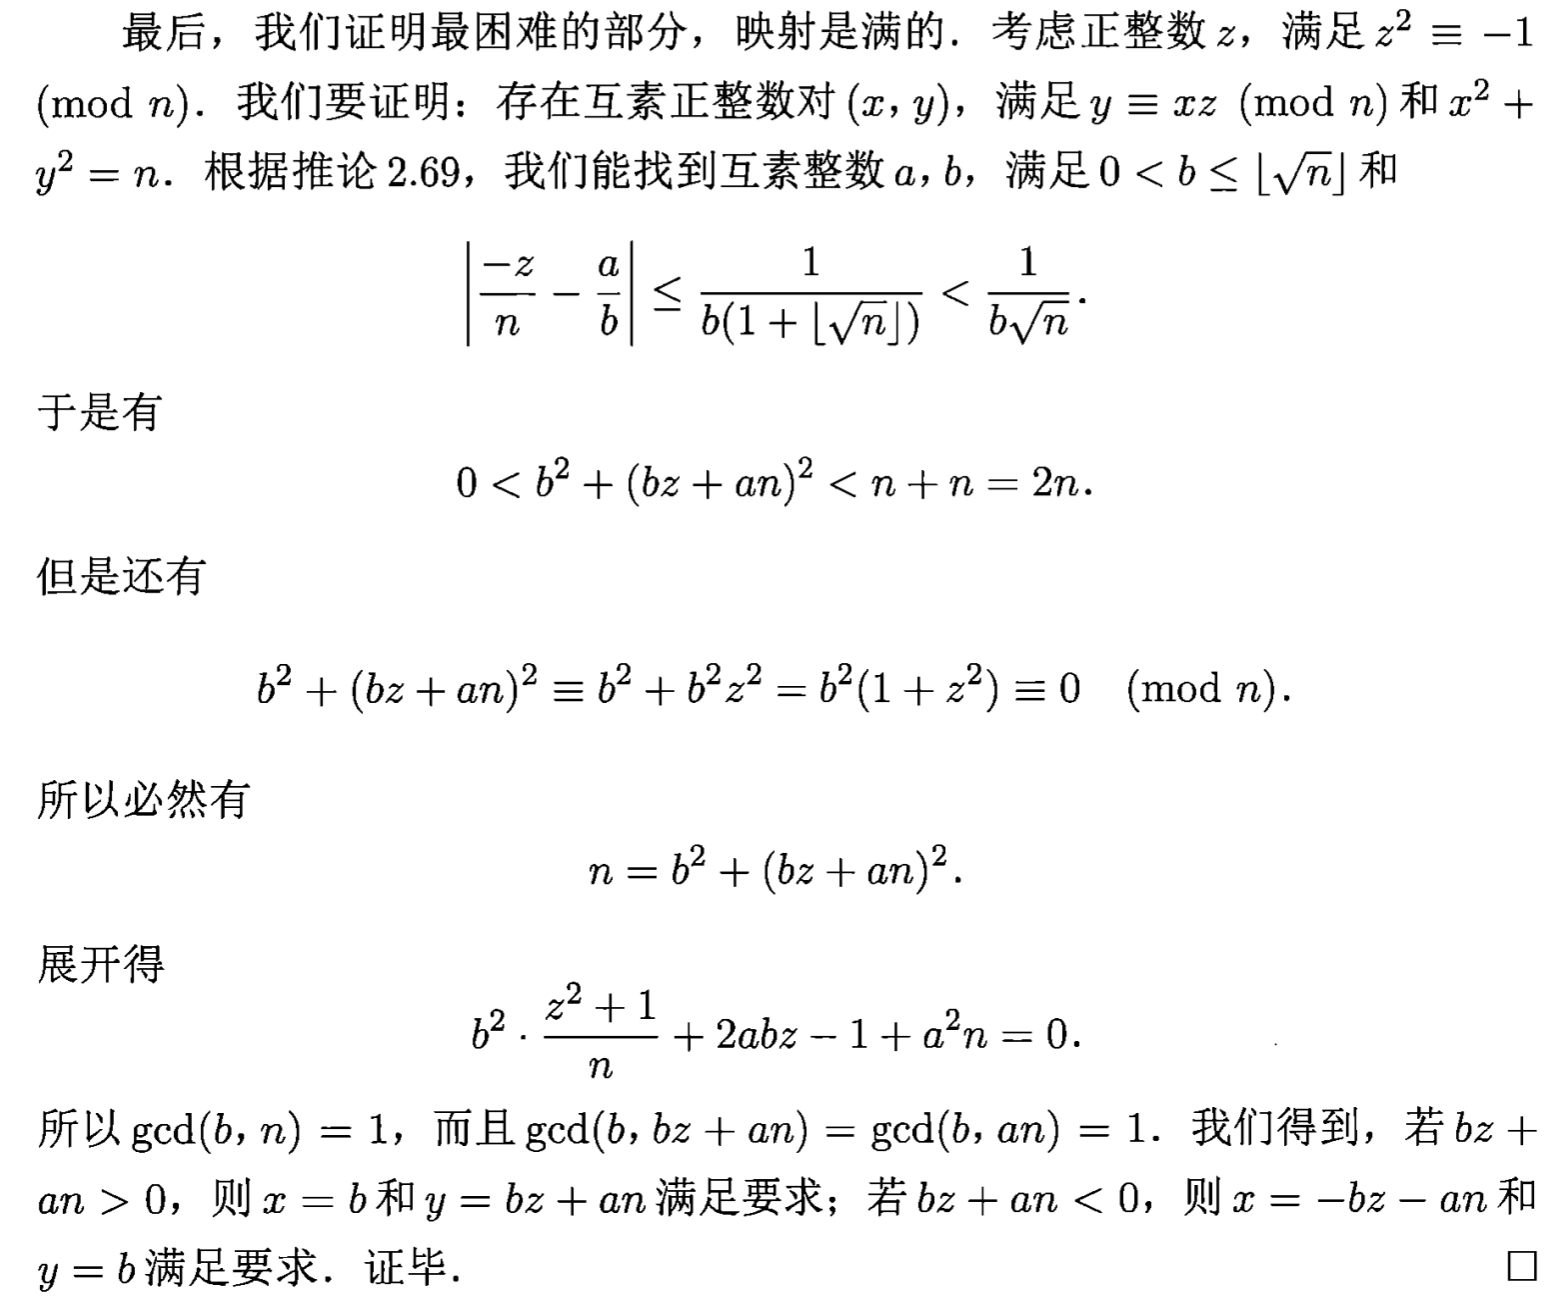
\includegraphics[width=13cm]{attachment/iShot_2024-01-06_21.42.59.png}
	\end{center}
	 
\end{proof}

\begin{theorem}{处理方程$x^2-dy^2=1$}
	设$d$是非平方正整数, 则方程$x^2-dy^2=1$存在正整数解. 
\end{theorem}
\begin{proof}
	给定$d$使得$\sqrt{d}$是无理数, 那么存在无穷多对$(x,y)$使得$|x-y\sqrt{d} |<\frac{1}{y}$, 特别地$$|x^2-dy^2| < \frac{1}{y}(x+y\sqrt{d}) < \frac{1}{y}(2y\sqrt{d} + \frac{1}{y}) < 3\sqrt{d}.$$
	所以存在(非零)整数$k$使得$x^2-dy^2=k$有无穷多对解. 
	
	\begin{center}
		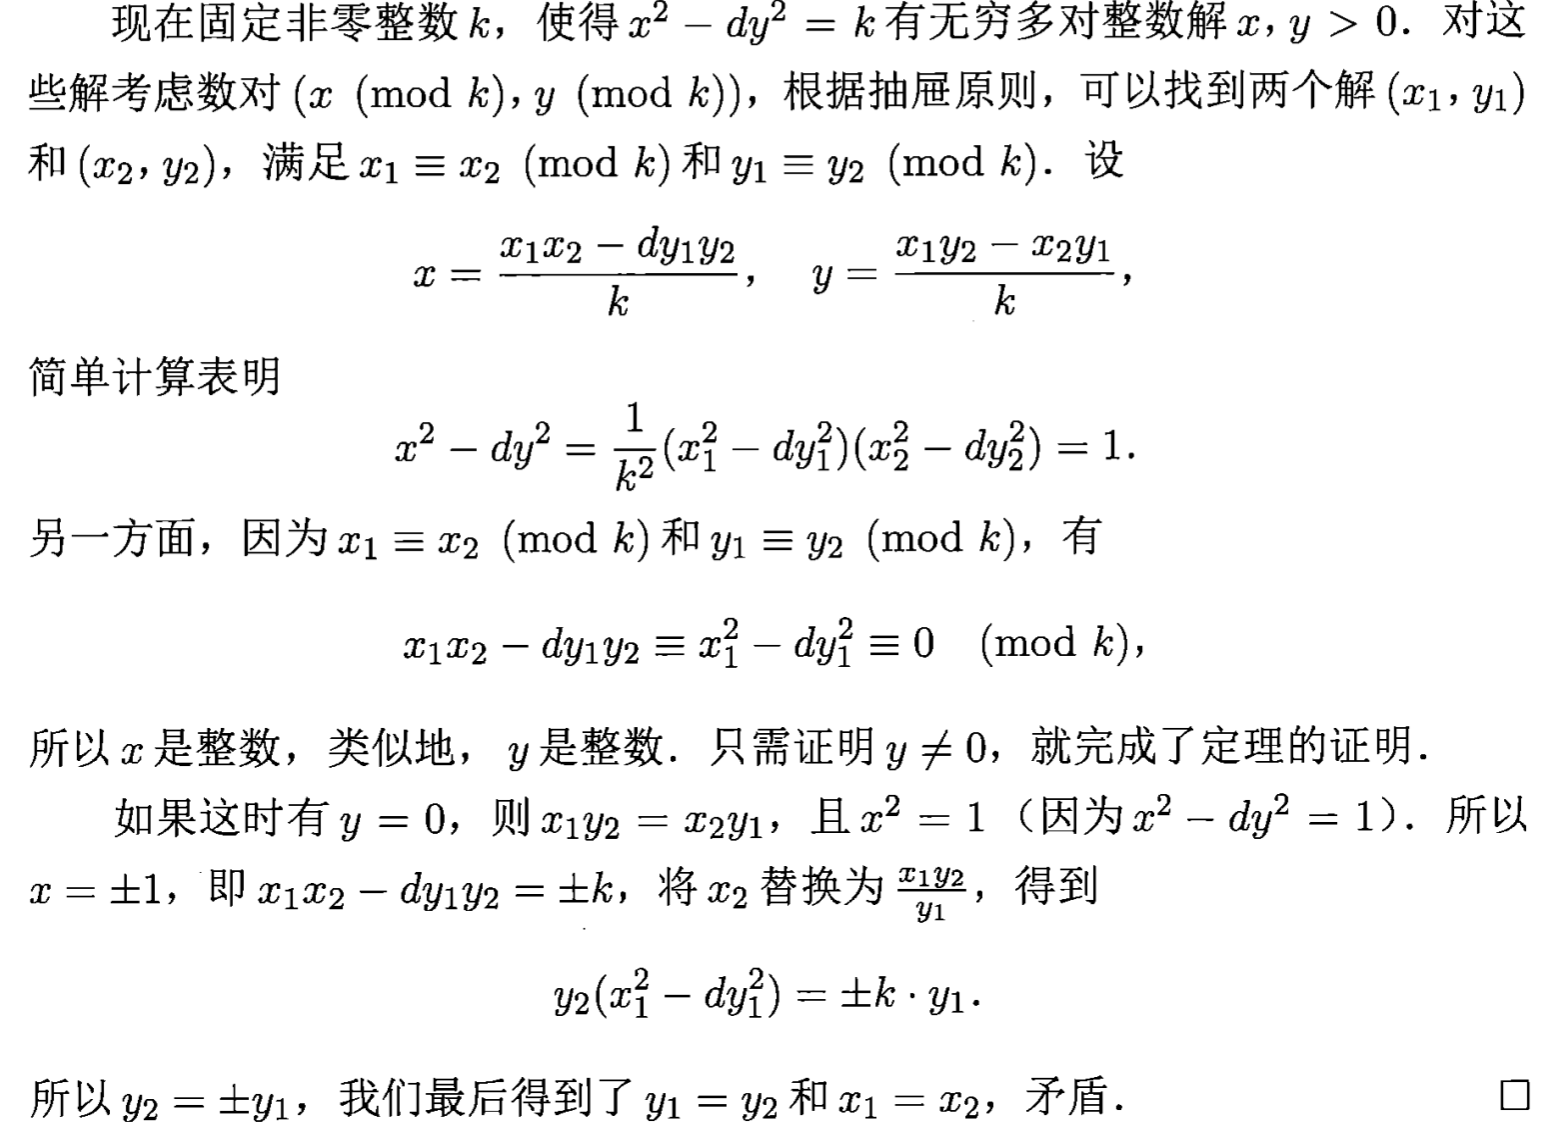
\includegraphics[width=13cm]{attachment/iShot_2024-01-06_21.53.15.png}
	\end{center}
\end{proof}

\subsection{连分数}

给定自然数序列$\{ q_n \}$, 定义序列$\{ R_n \}$: $$R_0=q_0, R_1=q_0+\frac{1}{q_1}, \cdots ,R_n = q_0 + \dfrac{1}{q_1 
          + \dfrac{1}{q_2 
          + \cdots \dfrac{1}{q_{n-1}+\dfrac{1}{q_n}}  } }.$$
我们也将$R_n$记作$[q_0;q_1,\cdots ,q_n]$. 


a) 对每个有理数$\frac{m}{l}$, 均存在唯一的$n$和$\{ q_n \}$使得$q_n \neq 1$且$R_n=\frac{m}{l}$. (提示: 利用Euclid算法)

b) 渐进分数序列$\{ R_n \}$满足以下不等式: $$\exists m,l,~ R_0<R_2< \cdots <R_{2k} < \frac{m}{l} < R_{2k+1} < R_{2k-1} < \cdots < R_1.$$

c) 每个无穷连分数(定义为数列$\{ R_n \}$的极限)都存在, 且为无理数. 

d) 可以按照如下方式递归地构造$R_k$的分子$P_k$与分母$Q_k$. 
$$P_0=q_0, P_1=q_0q_1+1, P_k=P_{k-1}q_k+P_{k-2}~(k \geq 2); $$
$$Q_0=1, Q_1=q_1, Q_k=Q_{k-1}q_k+Q_{k-2}~(k \geq 2).$$

e) 相邻两项渐进分数的差: $$\frac{P_{k+1}}{Q_{k+1}} - \frac{P_k}{Q_k} = \frac{(-1)^k}{Q_{k+1}Q_k}}. $$
\begin{proof}
	问题的关键是计算$P_{k+1}Q_k-Q_{k+1}P_k$. 实际上, $$P_{k+1}Q_k-Q_{k+1}P_k = (P_kq_{k+1}+P_{k-1})Q_k-(Q_kq_{k+1}+Q_{k-1})P_k = -(P_kQ_{k-1}-Q_kP_{k-1}) = \cdots = (-1)^k. $$
\end{proof}

f) 估计渐进分数的误差: 对于实数$x$和渐进分数序列$\{ \frac{P_n}{Q_n} \}$, $$\big| x-\frac{P_k}{Q_k} \big| \leq \frac{1}{Q_kQ_{k+1}} \leq \frac{1}{Q_k^2}. $$


\subsection{Pell方程}

\begin{theorem}{第一类Pell方程}
	设$(x_1,y_1)$是方程$x^2-dy^2=1$(其中$\sqrt{d}$是无理数)的最小解, 则一般解$(x_n,y_n)$有如下表达形式: 
	
	\begin{itemize}
		\item $x_n+y_n\sqrt{d} = (x_1+y_1\sqrt{d})^n$; 
		\item $x_{n+1}=x_1x_n+dy_1y_n,\qquad y_{n+1}=y_1x_n+x_1y_n$; 
		\item $x_{n+2}=(2x_1) x_{n+1}-x_n,\qquad y_{n+2} = (2x_1)y_{n+1}-y_n$; 
		\item $x_n = \frac{1}{2}\ssb{(x_1+y_1\sqrt{d})^n + (x_1-y_1\sqrt{d})^n},\qquad y_n = \frac{1}{2\sqrt{d}}\ssb{(x_1+y_1\sqrt{d})^n - (x_1-y_1\sqrt{d})^n}$; 
		\item 设$\sqrt{d}$的循环连分数周期为$\ell$, 渐进分数为$\{ \frac{P_n}{Q_n} \}$. 则$$(x_n,y_n) = \begin{cases}
 (P_{n\ell-1},Q_{n\ell -1}), & \text{ if } 2 \mid \ell \\
 (P_{2n\ell-1},Q_{2n\ell -1}).  & \text{ if } 2 \nmid \ell
\end{cases}$$
	\end{itemize}
\end{theorem}
\begin{proof}
	(1) 先证明第一种表示形式. 
	
	首先, 容易验证若$x_n+y_n\sqrt{d} = (x_1+y_1\sqrt{d})^n$, 由二项式定理我们有$x_n-y_n\sqrt{d} = (x_1-y_1\sqrt{d})^n$, 从而$$x_n^2-dy_n^2 = (x_1^2-dy_1^2)^n = 1.$$
	
	接着, 考虑方程的正整数解$(x,y)$. 记$z_1 = x_1+y_1 \sqrt{d}$, $z = x+y\sqrt{d}$. 由于$z \geq z_1$, 存在正整数$n$使得$z_1^n \leq z < z_1^{n+1}$. 计算$$\frac{z}{z_1^n} = (x+y\sqrt{d})(x_1-y_1\sqrt{d})^n =: u+v\sqrt{d},\qquad (x-y\sqrt{d})(x_1+y_1\sqrt{d})^n = u-v\sqrt{d}. $$
	注意到$u^2-dv^2 = (x^2-dy^2)(x_1^2-dy_1^2)^n = 1$. 现在$1 \leq u+v\sqrt{d} < z_1$, 假设$u+v\sqrt{d} > 1 > u-v\sqrt{d} >0$, 显然$u>0,v>0$. 从而我们得到了比$(x_1,y_1)$更小的解$(u,v)$, 矛盾. 因此$z = z_1^n$. 
	
	(2) 从(1)的证明中自然有第二条和第四条, 由第四条又可以得到第三条(利用线性递推公式)和第五条(此处略). 
\end{proof}
\vspace{1em}

\noindent
\textbf{\color{example} 例2.77.}~是否存在整数$a,b>1$, 使得$ab+1$和$ab^3+1$都是平方数? 
\vspace{1em}

接下来处理$ax^2-by^2=1$, 其中$a,b$为正整数. 特别地, 当$ab>1$是平方数时方程无正整数解. 
\vspace{1em}

\noindent
\textbf{\color{example} 例2.79.}~证明: 不存在正整数$a,b$使得$2a^2+1,2b^2+1,2(ab)^2+1$都是平方数. 

\begin{theorem}{}
	设正整数$a,b$满足$ab>1$不是平方数. 设$(x_1,y_1)$是方程$ax^2-by^2=1$的最小正整数解, $(u_n,v_n)$是方程$u^2-abv^2=1$的一般正整数解. 设方程$ax^2-by^2=1$的一般正整数解为$(x_n,y_n)$, 则: 
	
	\begin{itemize}
		\item $x_n=x_1u_n+by_1v_n,\qquad y_n=y_1u_n+ax_1x_n$; 
		\item $x_{n+2} = 2u_1x_{n+1}-x_n,\qquad y_{n+2} = 2u_1y_{n+1}-y_n$. 
	\end{itemize}
\end{theorem}

\begin{proposition}{两类Pell方程最小解的联系}
	设正整数$d$不是平方数, 使得方程$x^2-dy^2=-1$有正整数解. 设$(x_0,y_0)$是最小的正整数解, 则$(x_1,y_1)$满足$x_1+y_1\sqrt{d} = (x_0+y_0\sqrt{d})^2$是方程$x^2-dy^2=1$的最小正整数解. 
\end{proposition}
\begin{proof}
	记$(x_2,y_2)$是$x^2-dy^2=1$的最小整数解, $z_i=x_i+y_i\sqrt{d}$. 由上方定理可知, 存在正整数$n$使得$z_1=z_0^2=z_2^n$, 我们需要$n=1$, 即$n \geq 2$会得到$z_2^n \geq z_2^2 > z_0^2$矛盾, 于是只需证明$z_2>z_0$. 若不然, 计算$$\frac{z_0}{z_2} = (x_0+y_0\sqrt{d})(x_2-y_2\sqrt{d})=:u+v\sqrt{d} \quad \Rightarrow \quad u^2-dv^2=(x_0^2-dy_0^2)(x_2^2-dy_2^2)=-1. $$
	注意此时$z_0>u+v\sqrt{d}>1$, $0>u-v\sqrt{d}>-1$, 容易说明$u,v>0$, 从而得到矛盾. 
\end{proof}
\vspace{1em}

\noindent
\textbf{\color{example} 例2.82.}~求所有的正整数$m,n$, 使得$3^m = 2n^2+1$. 
\vspace{1em}

\noindent
\textbf{\color{example} 例2.83.}~证明: 存在无穷多个正整数$n$, 使得$n^2+1$有两个相差为$n$的正因子. 
\vspace{1em}

\noindent
\textbf{\color{example} 例2.84.}~证明: 存在无穷多对正整数组$(a,b,c)$构成等差数列且$ab+1,bc+1,ca+1$均为平方数. 


\vspace{2em}

由$\sum_{n & = 1}^{\infty}a_n$收敛, 可知任取$\varepsilon >0$, 存在$N>0$使得所有$n>N$和任意$p\geq 0$有$$(p+1)a_{n+p} \leq |a_n+\cdots +a_{n+p}| < \varepsilon .$$
固定$n$, 可知$\lim_{p\to \infty} (n+p)a_{n+p} = (n-1)\lim_{p\to \infty} a_{n+p} = 0$. 

















% Appendices section.
% \appendix

% Include the "about" appendix from the BackMatter subfolder.
% \chapter{About the Authors}

\section{First Author}

\blindtext

\section{Second Author}

\blindtext

% Include the "abbreviation" appendix from the BackMatter subfolder.
% \chapter{Abbreviations}

\blindtext

% Include the "notation" appendix from the BackMatter subfolder.
% \chapter{Notation}

\blindtext

% Include the "code" appendix from the BackMatter subfolder.
% \chapter{Supplementary Scripts}

\blindtext

% Include the "glossary" appendix from the BackMatter subfolder.
% \chapter{Glossary}

\blindtext

% Include the "index" appendix from the BackMatter subfolder.
% \chapter{Index}

\blindtext

% Include the "references" appendix from the BackMatter subfolder.
% \bibliography{references.bib}
\bibliographystyle{ieeetr}
\nocite{*}

% End the document.
\end{document}
